\documentclass[tg]{mdtufsm}
% * <routmagno@gmail.com> 2018-05-17T18:40:42.688Z:
%
% ^.
\usepackage{caption}
\usepackage[lofdepth,lotdepth,position=bottom]{subfig}
\captionsetup{
	justification=raggedright,
	figurewithout,labelsep=endash,
	singlelinecheck=false,compatibility=false
	}


%variaveis
\newcommand\numpartidas{230000}
\newcommand\partidasrankeds{197000}


%biblioteca para os grafos%
\usepackage{tikz}
\usetikzlibrary{shapes,arrows,matrix,positioning,backgrounds,calc}
\usetikzlibrary{plotmarks,patterns}
\usetikzlibrary{positioning}
\tikzset{main node/.style={circle,fill=orange!20,draw,minimum size=1cm,inner sep=0pt},
}
\tikzstyle{offnode}=[circle,fill=white!20,draw,minimum size=1cm,inner sep=0pt]
\tikzstyle{targetnode}=[circle,fill=blue!20,draw,minimum size=1cm,inner sep=0pt]
\tikzstyle{offline}=[gray, thick, dashed]

\renewcommand{\bf}{\bfseries}
%tabelas

\usepackage{booktabs}
\usepackage{multirow}
\usepackage{graphicx}
%\usepackage{subcaption}

\usepackage{chngcntr}
\counterwithout{figure}{chapter}
\counterwithout{table}{chapter}
\usepackage{ragged2e}
\usepackage{colortbl}
\usepackage{times}              % pacote para usar fonte Adobe Times
\usepackage{setspace}
\usepackage{array,multirow}
\usepackage{float}
\usepackage{siunitx}
\usepackage[portuguese,titlenumbered,ruled]{algorithm2e} % algoritmos
\usepackage[T1]{fontenc}        % pacote para conj. de caracteres correto
\usepackage{fix-cm} %para funcionar corretamente o tamanho das fontes da capa

\usepackage{times, color, xcolor}       % pacote para usar fonte Adobe Times e cores
\usepackage[utf8]{inputenc}   % pacote para acentuação
\usepackage{graphicx}  % pacote para importar figuras
\usepackage{amsmath,latexsym,amssymb} %Pacotes matemáticos
\usepackage[%hidelinks%, 
            bookmarksopen=true,linktocpage,colorlinks=true,
            linkcolor=black,citecolor=black,filecolor=magenta,urlcolor=blue,
            pdftitle={Título do Trabalho},
            pdfauthor={nome do autor},
            pdfsubject={Trabalho de Conclusão de Curso},
            pdfkeywords={modelo, latex, tcc, graduação}
            ]{hyperref} 

%Margens conforme MDT 2015
\usepackage[inner=30mm,outer=20mm,top=30mm,bottom=20mm]{geometry} 



%==============================================================================
% Se o pacote hyperref foi carregado a linha abaixo corrige um bug na hora
% de montar o sumário da lista de figuras e tabelas
% Se o pacote não foi carregado, comentar a linha %
%==============================================================================
%%=============================================================================
%% Trampa para corrigir o bug do hyperref que redefine o caption das figuras e das
%% tabelas, não colocando o nome ``Figura'' antes do número do mesmo na lista
%%=============================================================================

\makeatletter

\long\def\@caption#1[#2]#3{%
  \expandafter\ifx\csname if@capstart\expandafter\endcsname
                  \csname iftrue\endcsname
    \global\let\@currentHref\hc@currentHref
  \else
    \hyper@makecurrent{\@captype}%
  \fi
  \@ifundefined{NR@gettitle}{%
    \def\@currentlabelname{#2}%
  }{%
    \NR@gettitle{#2}%
  }%
  \par\addcontentsline{\csname ext@#1\endcsname}{#1}{%
    \protect\numberline{\csname fnum@#1\endcsname ~-- }{\ignorespaces #2}%
  }%
  \begingroup
    \@parboxrestore
    \if@minipage
      \@setminipage
    \fi
    \normalsize
    \expandafter\ifx\csname if@capstart\expandafter\endcsname
                    \csname iftrue\endcsname
      \global\@capstartfalse
      \@makecaption{\csname fnum@#1\endcsname}{\ignorespaces#3}%
    \else
      \@makecaption{\csname fnum@#1\endcsname}{%
        \ignorespaces
        \ifHy@nesting
          \expandafter\hyper@@anchor\expandafter{\@currentHref}{#3}%
        \else
          \Hy@raisedlink{%
            \expandafter\hyper@@anchor\expandafter{%
              \@currentHref
            }{\relax}%
          }%
          #3%
        \fi
      }%
    \fi
    \par
  \endgroup
}

\makeatother

%==============================================================================
% Identificação do trabalho
%==============================================================================
\title{Visualização e Classificação de uma rede complexa, e predição do resultado utilizando MLP: Analise do jogo \textit{League of Legends}. }

\author{Magno}{Guilherme}
%Descomentar se for uma "autora"
%\autoratrue

%% Lombada
\titulacao{Bacharel} %Tecn\'{o}logo ou Bacharel ou Licenciatura


\SetKwComment{Comment}{/*}{*/}
%folha rosto
\course{Bacharelado em Engenharia de Computação}
\initials{ENG COMP} 
\institute{Centro de Tecnologia}
\degree{Bacharel em Engenharia de Computação}

\faculdade{Instituto Federal de Minas Gerais}
\faculdadeing{Instituto Federal de Minas Gerais}
\siglafaculdade{IFMG}
\campus{Bambuí}

\cidade{Bambuí}
\siglaestado{MG}
\pais{Brasil}


% Número do TG (verificar na secretaria do curso)
% Para mestrado deixar sem opção dentro do {}
\trabalhoNumero{}

%Orientador
\advisoronepage[Prof.]{Dr.}{Mateus}{Laerte}
\advisor[Prof.]{Dr. (UFSM)}{TEM Q CONFERIR ISSO}{Nome do orientador}
%Se for uma ``orientadora'' descomentar a linha baixo
%\orientadoratrue

%Co orientador, comentar se não existir
%\coadvisor[Prof.]{Drª.}{Pereira}{Maria Regina}
%\coorientadoratrue %Se for uma ``Co-Orientadora''

%Avaliadores (Banca)
\committee[Me.]{Sobre nome}{Nome menbro banca}{UFSM}
\committee[Tecg.]{Sobre nome}{Nome menbro banca}{UFSM}

% a data deve ser a da defesa; 
% dia, mes e ano correntes
\date{dia}{mês}{2018} 

%Palavras chave
\keyword{modelo}
\keyword{latex} 
\keyword{tcc}
\keyword{graduação}

%keyword
\keywordAbstract{model}
\keywordAbstract{latex}
\keywordAbstract{tcc}
\keywordAbstract{graduation}
%%=============================================================================
%% Início do documento
%%=============================================================================
\begin{document}
	
	

%%=============================================================================
%% Capa e folha de rosto
%%=============================================================================
\maketitle
%%=============================================================================
%% Catalogação (obrigatório para mestrado) e Folha de aprovação
%%=============================================================================
%Somente obrigatório para dissertação, para TG, remover as linhas	77	%
%Como a CIP vai ser impressa atrás da página de rosto, as margens inner e outer	
%devem ser invertidas.

\newgeometry{inner=20mm,outer=30mm,top=30mm,bottom=20mm}	
\makeCIP{Routmagno@gmail.com} %email do autor		
\restoregeometry

%Se for usar a catalogação gerada pelo gerador do site da biblioteca comentar as linhas
%\includeCIP{CIP.pdf}
	
%%=============================================================================
%folha de aprovação
%%=============================================================================
\makeapprove

%%=============================================================================
%% Dedicatória (opcional)
%%=============================================================================
\chapter*{Dedicatória}


\vfill

\begin{center}
	
	{\sffamily\itshape Dedico este trabalho a ......}
	
\end{center}

\vfill

\newpage
%%=============================================================================
%% Agradecimentos (opcional)
%%=============================================================================
\chapter*{Agradecimentos}


\justifying{\textit{Agradeço .....}}



%%=============================================================================
%% Epígrafe (opcional)
%%=============================================================================
\clearpage
\begin{flushright}
\mbox{}\vfill

{\sffamily\itshape
	\begin{quote}
		\begin{quote}
			\begin{quotation}
			``O valor de uma coisa depende da maneira como a abordamos mentalmente e não da coisa em si'' \\
			
			\begin{flushright}
			\textsc{(Jigoro Kano)}
		  	\end{flushright}
		  	
		\end{quotation}
		\end{quote}
	\end{quote}
 }




\end{flushright}

%%=============================================================================
%% Resumo
%%=============================================================================
\begin{abstract}
		
Aqui você escreve o resumo. Lembrando no máximo 250 palavras para tcc e 500 palavras para tese ou dissertação.

\end{abstract}

%%=============================================================================
%% Abstract
%%=============================================================================
% resumo na outra língua
% como parametros devem ser passados o titulo, o nome do curso,
% as palavras-chave na outra língua, separadas por vírgulas, o mês em inglês
%o a sigla do dia em inglês: st, nd, th ...
\begin{englishabstract}
{Abstract title}
%%============ MANTER ESSA LINHA ============================================
\ %%============ MANTER ESSA LINHA ==========================================
%%============ MANTER ESSA LINHA ============================================
\ %%============ MANTER ESSA LINHA ==========================================
%%============ MANTER ESSA LINHA ============================================
\ %%============ MANTER ESSA LINHA e deixar uma em branco ===================


Here you write the summary. Remembering a maximum of 250 words for tcc and 500 words for thesis or dissertation.

\end{englishabstract}

%% Lista de Ilustrações (opc)
%% Lista de Símbolos (opc)
%% Lista de Anexos e Apêndices (opc)

%%=============================================================================
%% Lista de figuras (comentar se não houver)
%%=============================================================================
\listoffigures
%%=============================================================================
%% Lista de tabelas (comentar se não houver)
%%=============================================================================
\listoftables

%%=============================================================================
%% Lista de Apêndices (comentar se não houver)
%%=============================================================================
%\listofappendix

%%=============================================================================
%% Lista de Anexos (comentar se não houver)
%%=============================================================================
%\listofannex

%%=============================================================================
%% Lista de abreviaturas e siglas
%%=============================================================================
 %o parametro deve ser a abreviatura mais longa

\begin{listofabbrv}{UbiComp}
	

	  \item [MOBA]        Arena de batalha online de multijogadores ( do inglês \textit{Multiplayer Online Battle Arena} )

  	\item [API]        Interface de Programação de Aplicativos ( do inglês \textit{Application Programming Interface} )
  	\item [JSON]        Notação de Objeto JavaScript ( do inglês \textit{ JavaScript Object Notation} )
  	\item [URL]        Localizador Uniforme de Recursos ( do inglês \textit{Uniform Resource Locator} )
  	\item [MLP]        Perceptron Multicamadas ( do inglês \textit{Multilayer Perceptron} )
  	\item [LOL]	 Liga das Lendas ( do inglês \textit{League of Legends})
  	\item [IFMG]	 Instituto Federal de Minas Gerais
    
\end{listofabbrv}

%%=============================================================================
%% Lista de simbolos (opcional)
%%=============================================================================
%Simbolos devem aparecer conforme a ordem em que aparecem no texto
% o parametro deve ser o símbolo mais longo
%\begin{listofsymbols}{teste}
%  \item [$\varnothing$] vazio
 % \item [$\Gamma$]  Gama
%  \item [$\forall$] Para todo
%\end{listofsymbols}

%%=============================================================================
%% Sumário
%%=============================================================================
\tableofcontents











%%=============================================================================
%% Início da dissertação
%%=============================================================================
\setlength{\baselineskip}{1.5\baselineskip}

%Adiciona cada capitulo
\chapter{Introdução}
\label{chap:Introducao}

Muitos pesquisadores tem tido interesse em estudar sobre grafos, pois estes estão sendo desenvolvidos para modelizar sistemas \cite{joachim}, como, por exemplo, rede de energia de Nova York e a rede alimentar de Little Rock Lake \cite{strogatz}.
Os objetivos desses pesquisadores são variados, que podem ser desde classificação de grafos \cite{fbclass}, à predição \cite{dota} e para uma compreensão melhor do mesmo \cite{rosvall2008maps}. 

Alguns exemplos de modelação das pesquisas são redes sociais \cite{fbclass}, estruturas químicas \cite{rosvall2008maps} e jogos \cite{dota}. Em nosso trabalho, trabalharemos na de jogos, pois ainda no meio acadêmico são novidades quando se trata de modelação em grafos.
Jogos que tem conquistado a atenção e o tempo de muitas pessoas, movimentando mais receita do que a industria de filmes Hollywood\footnote{http://www.webnoticias.fic.ufg.br/n/68881-industria-de-games-supera-o-faturamento-de-hollywood}.

Com a popularização do \textit{\textbf{L}eague \textbf{o}f \textbf{L}egends}\footnote{https://play.br.leagueoflegends.com/pt\_BR}, também conhecido como LOL, um jogo da categoria de MOBA (\textbf{M}ultiplayer \textbf{O}nline \textbf{B}attle \textbf{A}rena, ou, pela tradução, "Arena de batalha online de multijogadores"), e sua crescente premiação em campeonatos\footnote{http://www.espn.com.br/noticia/736116\_premiacao-do-mundial-de-league-of-legends-ultrapassa-us-4-milhoes}, jovens e adultos tem se tornado \textit{pro players} (de tradução: jogadores profissionais) e dedicado sua vida ao mundo dos jogos\footnote{https://oglobo.globo.com/esportes/de-nerds-ciberatletas-crescimento-exponencial-do-sports-21233721}. 
Esse fato viabiliza o uso de ferramentas para ajudá-los na análise dos jogos e de estratégias. 
Devido a popularidade do jogo e a facilidade de obtenção dos dados devido a API ( \textbf{A}pplication \textbf{P}rogramming \textbf{I}nterface ou, da tradução, Interface de Programação de Aplicações) do LOL, ele é escolhido como foco do trabalho.

Nesse contexto, o presente trabalho propõe a modelagem do grafo das partidas do jogo \textit{League of Legends}, a sua visualização, a classificação do mesmo e a predição de equipes vencedoras utilizando MLP (Multilayer Perceptron, ou, da tradução, Perceptron Multicamadas), no formato de um \textit{webservice} (da tradução, serviço da internet).

\section{Contextualização}
Na matriz curricular do curso de Engenharia de Computação do Instituto Federal de Minas Gerais - \textit{campus} Bambuí, existem várias disciplinas que foram utilizadas no presente trabalho (como Programação Orientada a Objetos, Banco de Dados, Programação Web dentre outras) e com o estudo mais aprofundado sobre grafos, foi possível desenvolver o \textit{webservice} pois a API do LOL é fácil de ser usada e facilita a obtenção dos dados.


A proposta deste trabalho será o desenvolvimento de um \textit{webservice} que indicará uma possível equipe vencedora, de acordo pela escolha dos campeões (personagens jogáveis do jogo, em que cada um, individualmente, tem atributos e habilidades diferentes) dos jogadores, e, também, mostrar a sinergia entre os campeões e o seus \textit{counter picks} (da tradução, "contra-escolha", que seria uma expressão usada nos jogos de MOBA para indicar quando um campeão específico tem, por sí só, uma vantagem sobre outro campeão, também específico). Também será feito a classificação da modelação do grafo obtido dos dados do jogo para fins acadêmicos.

\section{Objetivos}
\subsection{Objetivos Gerais}
Criar um modelo computacional capaz de exibir resumos da rede complexa gerada dos dados armazenados e predizer um vencedor no jogo \textit{League of Legends} baseando-se num histórico de partidas usando MLP.

\subsection{Objetivos Específicos e Resultados Esperados}

\begin{enumerate}
\item Construir um \textit{webservice} para visualização;
\item Calcular deterministicamente quantas vezes cada herói ganhou contra/com outro herói;
\item Classificar o grafo;
\item Testar o resultado obtido em outra amostra de dados;
\item Documentar os resultados.

\end{enumerate}

\section{Justificativa}
Devido ao grande crescimento e a popularização do jogo \textit{League of Legends}, tem surgido muitos sites de análises do mesmo que vem auxiliando tanto os jogadores esporádicos, tanto quanto os \textit{pro players}.
Este trabalho propõe desenvolver um modelo computacional para que usuários, \textit{coach}, ou analistas possam ter uma ferramenta para obtenção de informações ou para predição do resultado de um jogo.

A utilização da rede complexa para modelar os dados, foi escolhida, pois ela possibilita representar quantificadamente as conexões de cada herói, sendo conexões aliadas ou adversárias.

Assim, este trabalho se justifica principalmente pela análise da rede complexa obtida, pela visualização gráfica e pela predição de partidas para que estas informações adquiridas se tornem acessíveis. 
Para execução desse trabalho é necessário o uso de várias áreas do conhecimento estudadas no curso de Engenharia de Computação, principalmente computação.
\chapter{Fundamentação Teórica}
\label{chap:fundteorica}
Nessa parte será apresentados conceitos para melhor entendimento deste trabalho e da modelação utilizada. 
A seção \ref{chap:grafos} elucida o que são grafos e o capítulo \ref{chap:redecomplexa} explica a variação de grafo utilizado para modelar o problema proposto. Depois na seção \ref{chap:lol} é esclarecido o ambiente que será abstraído, explicando algumas regras básicas do jogo.
\section{Grafos}
\label{chap:grafos}

Quando descrevemos uma situação utilizando pontos e ligações entre algum desses pontos, como o exemplo os pontos sendo pessoas e as ligações entre as pessoas sendo as amizades feitas, a abstração matemática desse tipo dá lugar ao conceito de grafo \cite{Lucchesi1979}.

Segundo \citet{Viana2007} "Um grafo \(G(V, E)\) pode ser definido como um conjunto de vértices \(V\), e um conjunto de conexões \(E\) " e ele continua: "Cada elemento do conjunto \(E\), associa dois elementos do conjunto \(V\), assim, se \((u,v) \in E\), então existe uma conexão entre os vértices u e o vértice v .". Sendo eles classificados como vizinhos ou adjacente \cite{grafosucinto}.


\subsection{Binário e Não-binário}
Os grafos também podem ser classificados como binários e não-binários, sendo os binários suas arestas representadas por 1 ( se existem ) ou 0 ( se não existem ) e os não-binários quando existe um conjunto \(W\) onde informa a intensidade da interação de uma aresta entre dois vértices  \cite{Viana2007}.
Na Figura \ref{fig:grafo-exemplobinario} temos um grafo binário onde se \((u,v) \in E\) então ela está representada no grafo, já na Figura \ref{fig:grafo-exemplonaobinario} além da existência da conexão entre os vértices, está representado o conjunto \(W\) informando o peso ou aresta daquela aresta.

\begin{figure}[!h] \centering
	\centering
	\caption{Exemplo de grafos.}
	\subfloat[Grafo binário com quatro vértices e quatro arestas.]{
		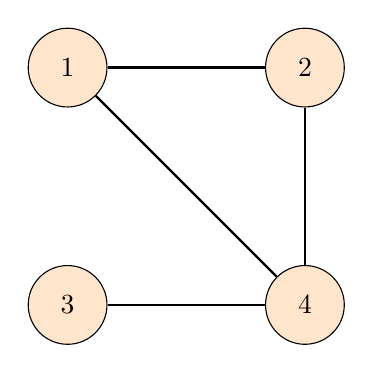
\begin{tikzpicture}
		\begin{scope}[xshift=4cm]
		\node[main node] (1) {$1$};
		\node[main node] (2) [right = 2cm  of 1] {$2$};
		\node[main node] (3) [below = 2cm  of 1] {$3$};
		\node[main node] (4) [right = 2cm  of 3] {$4$};
		
		\path[draw,thick]
		(1) edge node {} (2)
		(1) edge node {} (4)
		(4) edge node {} (2)
		(4) edge node {} (3)
		;
		\end{scope}
		\end{tikzpicture}
		\label{fig:grafo-exemplobinario}
	}
	\subfloat[Grafo não-binário com quatro vértices e três arestas.]{
		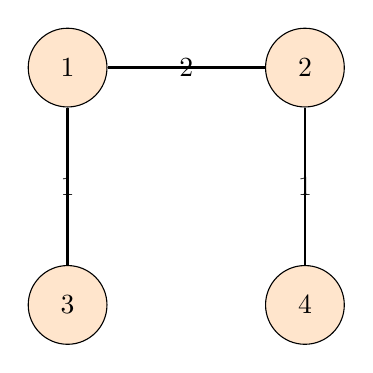
\begin{tikzpicture}
		\begin{scope}[xshift=4cm]
		\node[main node] (1) {$1$};
		\node[main node] (2) [right = 2cm  of 1] {$2$};
		\node[main node] (3) [below = 2cm  of 1] {$3$};
		\node[main node] (4) [right = 2cm  of 3] {$4$};
		
		\path[draw,thick]
		(1) edge node {2} (2)
		(1) edge node {1} (3)
		(2) edge node {1} (4)
		;
		\end{scope}
		\end{tikzpicture}
		\label{fig:grafo-exemplonaobinario}
	}
	\
	\small{\leftline{Fonte: Autor.}}
	\label{fig:grafo-exemplo}
\end{figure}


\subsection{Vizinhança}
\citet{grafosucinto} diz sobre a vizinhança de um grafo que "O conjunto de vértices \(X\) de um grafo \(G\) é o conjunto de todos os vértices que tem algum vizinho em \(X\)", e diz que esse conjunto de vértices pode ser chamado de \(\Gamma_G(X)\). Exemplificando, o conjunto \(\Gamma_G(1)\) da Figura \ref{fig:grafo-exemplobinario} são os vértices \(2\) e \(4\) e a aresta \( (2,4) \) sendo representados na Figura \ref{fig:grafo-vizinhanca}.

\begin{figure}[H] \centering
	\centering
	\caption{Exemplo de vizinhança de um vértice de um grafo.}
		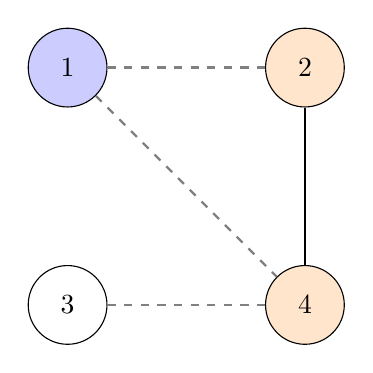
\begin{tikzpicture}
		\begin{scope}[xshift=4cm]
		\node[targetnode] (1) {$1$};
		\node[main node] (2) [right = 2cm  of 1] {$2$};
		\node[offnode] (3) [below = 2cm  of 1] {$3$};
		\node[main node] (4) [right = 2cm  of 3] {$4$};

		\path[draw, style={offline}]
		(1) edge node {} (2)
		(1) edge node {} (4)
		(3) edge node {} (4)
		;
		\path[draw,thick]
		(4) edge node {} (2)
		;
		\end{scope}
		\end{tikzpicture}
	\small{\leftline{Fonte: Autor.}}
	\label{fig:grafo-vizinhanca}
\end{figure}

\subsection{Grau}

O grau de um vértice \(v\) é definido por \citet{grafosucinto} sendo a quantidade de arestas que chegam no vértice \(v\), sendo denotado por \(g(v)\). Continuando ainda no exemplo da Figura \ref{fig:grafo-exemplobinario} o \(g(1)\) é 2 pois apenas as arestas \((1,2)\) e \((1,4)\) incidem no vértice 1.

O grau máximo de um grafo \(G\) é o número do vértice que tem o maior grau presente nesse grafo, ou seja \(\Delta(G) = max\{g(v) : v \in V(G)\}\). E o grau mínimo de um grafo \(G\) é o grau do vértice com menor grau, \(\delta(G) = min\{g(v) : v \in V(G)\}\). E ainda, um grafo é regular se \(\delta(G) = \Delta(G)\) e é \(k\)-regular se \(\delta(G) = \Delta(G) = k\) \cite{grafosucinto}.


E quando modelamos um sistema real em forma de grafos vamos ver na seção seguinte que esse grafo recebe um nome especial, sendo chamado de rede complexa.

\section{Redes Complexas}
\label{chap:redecomplexa}
Sobre redes complexas \citet{Viana2007} diz que é utilizado o termo redes complexas quando um grafo representa um sistema físico real, então levando em conta isso, um grafo do jogo LOL pode ser considerado como uma rede complexa.

Para que seja possível classificar os resultados adequadamente, serão apresentados três modelos que se destacam no estado da arte segundo \citet{Albert2002}: As redes \textit{small worlds}, as redes livres de escala e as redes aleatórias. E também será explicado sobre o coeficiente de aglomeração .

\subsection{\textit{Redes Small Worlds}}
 As redes \textit{small worlds} são redes que o caminho entre dois nós são relativamente pequenos. (continua...).
 
 
 \subsection{Redes Livres de Escala}
 Nas redes livres de escala um nó tem a probabilidade \(P(k)\) de possuir \(k\) arestas obedecendo a lei da potência \(P(k) \sim k^{-y}\) \cite{Albert2002,Antiqueira2005}. Segundo \citet{Viana2007} nas redes livres de escala muitos nós tem poucas arestas e poucos nós se ligam a muitos.
 
     
\subsection{Redes Aleatórias}
Segundo \citet{Viana2007} as redes aleatórias são um sistema formado por E arestas e N vértices, onde as arestas são distribuídas aleatoriamente. \citet{CunhaRecuero2004} apud ( tenho que ver certinho ) exemplifica esse tipo de rede como uma festa, onde “bastava uma conexão entre cada um dos convidados de uma festa, para que todos estivessem conectados ao final dela” e que quanto mais conexões forem criadas, maior a chance de serem criados grupos de pessoas que de tempos em tempos se relacionavam com outros grupos e que poderiam concluir que esses nós se relacionavam de forma randômica.

 
 \subsection{Coeficiente de Aglomeração}
 Segundo \citet{Viana2007} o coeficiente de aglomeração mede o quão conectado estão os nós da rede ou do grafo. \citet{Antiqueira2005}  define o coeficiente de aglomeração sendo:\[CA_i = \frac{E_i}{k_i(k_i-1)}\]


\citet{Antiqueira2005}  continua: “Sendo para cada vértice \(i\) existe \(k_i\) arestas, que os ligam a outros \(k_i\) vértices. Se esses \(k_i\) vértices estivessem ligados diretamente à todos os outros vértices do conjunto, haveriam \(k_i(k_i- 1)\) arestas entre eles. E assumindo \(E_i\) o número de arestas que existentes entre os \(k_i\) vértices.	O coeficiente da rede inteira é a média de todos \(CA_i\)”.

\begin{figure}[!h] \centering
	\centering
	\caption{Coeficiente de aglomeração.}
	\subfloat[]{
		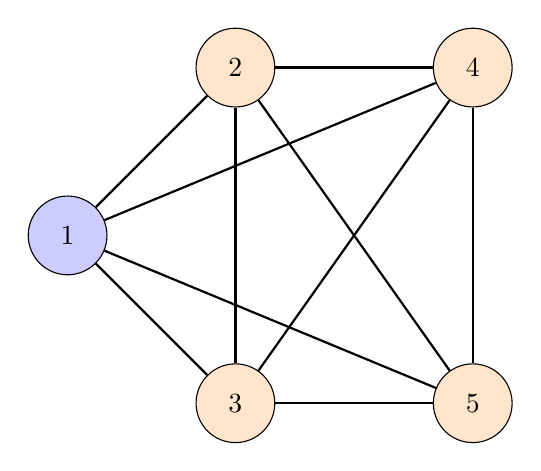
\begin{tikzpicture}
		\begin{scope}[xshift=4cm]
		\node[targetnode] (1) {$1$};
		\node[main node] (2) [above right = 2cm  of 1] {$2$};
		\node[main node] (3) [below right = 2cm  of 1] {$3$};
		\node[main node] (4) [right = 2cm  of 2] {$4$};
		\node[main node] (5) [right = 2cm  of 3] {$5$};
		
		\path[draw,thick]
		(1) edge node {} (2)
		(1) edge node {} (3)
		(1) edge node {} (4)
		(1) edge node {} (5)	
		(2) edge node {} (3)
		(2) edge node {} (4)
		(2) edge node {} (5)
		(3) edge node {} (4)
		(3) edge node {} (5)
		(4) edge node {} (5)
		;
		\end{scope}
		\end{tikzpicture}
		\label{fig:grafo-aglomeracao1}
	}
	\subfloat[]{
		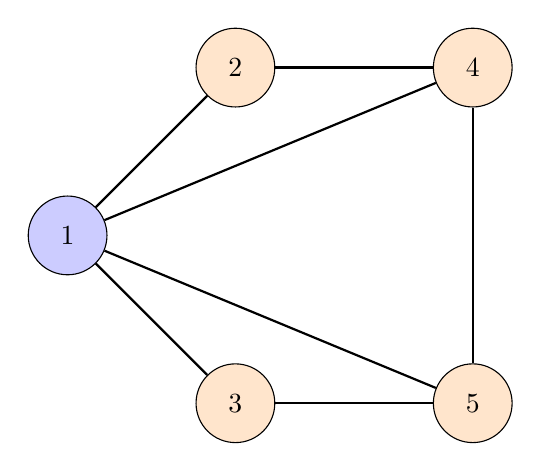
\begin{tikzpicture}
		\begin{scope}[xshift=4cm]
		\node[targetnode] (1) {$1$};
		\node[main node] (2) [above right = 2cm  of 1] {$2$};
		\node[main node] (3) [below right = 2cm  of 1] {$3$};
		\node[main node] (4) [right = 2cm  of 2] {$4$};
		\node[main node] (5) [right = 2cm  of 3] {$5$};
		
		\path[draw,thick]
		(1) edge node {} (2)
		(1) edge node {} (3)
		(1) edge node {} (4)
		(1) edge node {} (5)
		(2) edge node {} (4)
		(3) edge node {} (5)
		(4) edge node {} (5)
		;
		\end{scope}
		\end{tikzpicture}
		\label{fig:grafo-aglomeracao2}
	}
	\
	\small{\leftline{Fonte: Autor.}}
	\label{fig:grafo-aglomeracao}
\end{figure}

Na Figura \ref{fig:grafo-aglomeracao1}, assumindo o peso de todas as arestas como 1, o coeficiente de aglomeração do vértice em azul é 1, já na Figura \ref{fig:grafo-aglomeracao2} o coeficiente do vértice em azul segundo a fórmula é $\frac{1}{2}$. 
    


\section{\textit{League of Legends}}
\label{chap:lol}
O jogo \textit{League of Legends} é um jogo classificado como arena de batalha online de multi jogadores (do inglês \textit{Multiplayer Online Battle Arena} ) ou conhecido também como MOBA, que é um estilo de jogo onde duas equipes se enfrentam em um campo de batalha e cada jogador controla o seu personagem, mais chamado de herói ou campeão. O objetivo do MOBA é derrotar a equipe adversária destruindo a construção principal da equipe inimiga.

	A arena onde acontece o jogo é uma arena onde normalmente o mapa inicialmente é  espelhado,  ou  seja, o lado que cada time está não  oferece vantagens  exclusivas.  O mapa é composto  de  três caminhos até a base inimiga.
    
%%preciso conferir se essa foto é acervo, ou é do lol

\begin{figure}[H]
	\caption{Mapa do jogo de \textit{League of Legends}}
	\begin{center}
		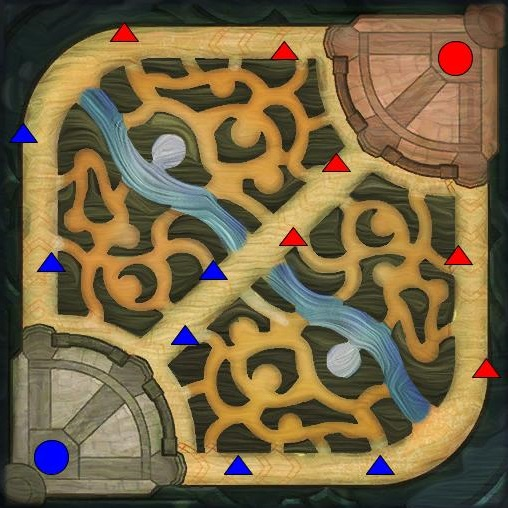
\includegraphics{imagens/mapa_lol.jpg}
	\end{center}
	\small{Fonte: Autor (2018).}
	\label{fig:mapa_lol}
\end{figure}

	A Figura \ref{fig:mapa_lol} mostra como é realmente o mapa do jogo, sendo que os círculos mostram a localização da construção principal, e os triângulos as construções de suporte de cada equipe, sendo azul uma equipe e vermelho a outra.
    
	Com o início do jogo cada jogador escolhe  um  herói  diferente, onde  cada  herói tem um conjunto de características únicas, como habilidades especiais,  seu impacto  no jogo,  na equipe adversária e na equipe aliada.
    
	Depois de escolher os heróis de cada equipe, cada jogador deve procurar adquirir recursos no jogo e objetivos para conseguir vantagens. Os recursos são limitados por equipe e por tempo, ou seja, deve ser bem escolhido quem ficará com a maior parte dos recursos da equipe.

\section{Estado da Arte}


{\Huge VOU REFAZER}


No estado da arte, estudos com jogos de gênero MOBA são poucos, mas relacionados a redes complexas e predição existem diversos.

\subsection{Identifying Patterns in Combat that are Predictive of success}
 O trabalho de Yang \textit{et al}, relacionou a posição dos jogadores em uma batalha do MOBA com redes complexas, ao predizer o time vencedor daquela batalha.

\begin{figure}[!ht]
	\caption{As estruturas gráficas de uma batalha de MOBA}
	\begin{center}
		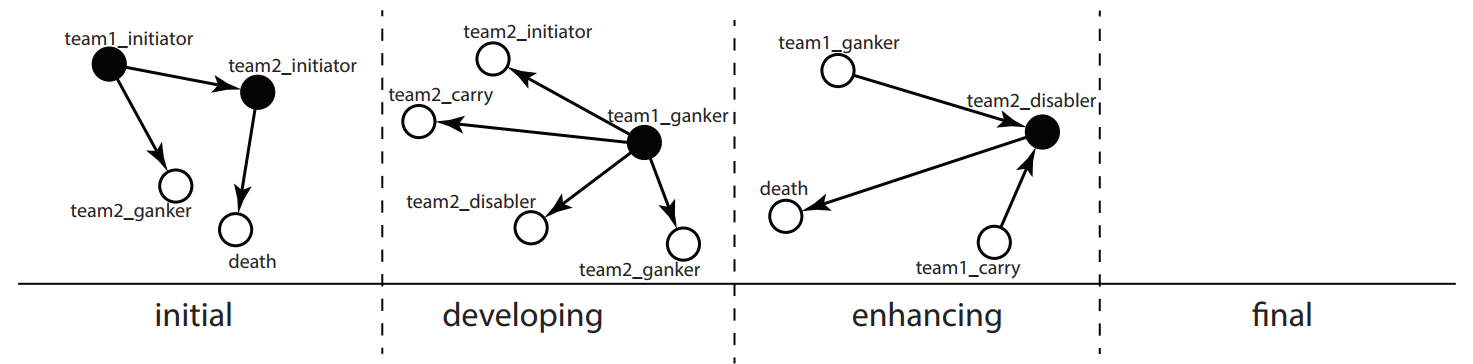
\includegraphics[width=15cm]{imagens/yang.PNG}
	\end{center}
	\small{Fonte: \cite{Yang2014}.}
	\label{fig:yang2014}
\end{figure}

Yang \textit{et al} modela os dados de um combate, em redes complexas, e treina uma arvore de decisão usando as melhores características tiradas dessa rede complexa. Depois de treinado a árvore, é identificado regras de combate que são preditivas de sucesso, e depois essas regras são traduzidas de volta em um padrão de combate específico usando uma técnica chamada mineração de subgrafo frequente.

\subsection{Análise de uma Métrica Alternativa para Predição de Laços Sociais em Grafos Lei de Potência}

Feito por \citeauthor{Danielewicz2016}, ela mostra uma visão geral do problema de predição de laços sociais, analisa os modelos de geração de grafos principalmente que seguem a lei da potência, no âmbito de formação de laços sociais e depois consegue uma métrica para predição de laços. Ela faz testes usando técnicas diferentes, mostrando seus resultados.
\chapter{Metodologia}
Este capítulo apresenta as ferramentas e algoritmos utilizados neste projeto, tanto no processo de extração do conhecimento, quanto na visualização dos dados.
A primeira seção irá explicar como os dados estão disponíveis na API da Riot Games e quais informações eles carregam. A segunda clarifica como estes dados serão armazenadas e a terceira fala de que maneira se processa os dados, verifica se os dados estão completos e armazena-os em um banco de dados.

\section{API}
A Riot Games, desenvolvedora e dono do jogo \textit{League of Legends}, fornece uma Interface de Programação de Aplicativos ( do inglês \textit{Application Programming Interface} ) ou chamado de API, para que terceiros consigam acessar dados sobre os jogos.

A Riot games disponibiliza o acesso as informações à patir da URL\footnote{http://developer.riotgames.com}, de modo que é gerado uma chave válida por 1 ano para projetos cadastrados.
O acesso à essa API é por URL utilizando uma função disponível pela Riot Games. Neste trabalho, usaremos apenas a função \textit{MATCH-V3} que é uma função que retorna os dados de uma partida já terminada.

A função \textit{MATCH-V3} é disponibilizada publicamente pela Riot Games, retornando um conjunto de informações no formato JSON sobre a partida passada por parâmetro, quando essa partida existe. A Figura \ref{fig:match-v3} resume um exemplo de uso da função acessando a URL\footnote{https://br1.api.riotgames.com/lol/match/v3/matches/1381102031?api\_key=minhachave}, acessada em 21 de março de 2018 pelo autor, sendo que \(minhachave\) tem que ser substituída por uma chave privada válida.
\begin{figure}[H]
	\caption{Exemplo de retorno do uso da função \textit{MATCH-V3}. Sendo as informações divididas em informações da partida, informações dos times e informações dos participantes.}
	\begin{center}
		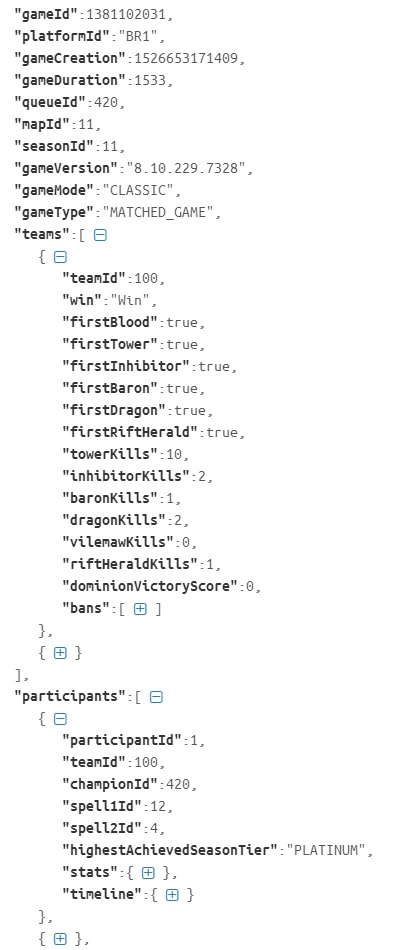
\includegraphics[width=9cm]{imagens/match-v3.jpg}
	\end{center}
	\small{Fonte: Autor.}
	\label{fig:match-v3}
\end{figure}

De todas essas informações retornadas pela função, as que foram armazenadas para o projeto por participante são:

\begin{enumerate}
\item \textit{gameId}. Identificador único da partida;
\item \textit{kills}, \textit{deaths} e \textit{assists}. Informações que falam, respectivamente, quantas vezes esse jogador matou, morreu e participou na morte de outrem;
\item \textit{win}. Se ele ganhou;
\item \textit{championId}. Qual campeão ele escolheu;
\item \textit{lane}. Em qual posição ele tava jogando;
\item \textit{platformId}. Em qual servidor ele jogava;
\item \textit{queueId}. E qual o tipo de partida.
\end{enumerate}

Sabendo qual informação vamos armazenar, ficou escolhido a linguagem \textit{Python} para ser desenvolvido o algoritmo no qual obterá as informações de forma não manual e o sistema de gerenciamento de banco de dados MySQL. Na próxima seção será apresentado sobre banco de dados e na seção \ref{chap:aquisicao} será esclarecido como foram obtidos o \textit{dataset} das partidas. 


\section{Persistência dos dados}
Os dados adquiridos serão armazenados em um banco de dados MySQL, cujo o esquema das tabelas podem ser vistas na Figura \ref{fig:bd}, onde é possível ver quais foram as informações salvas. Com o esquema do banco de dados pronto, já é possível passar para a aquisição dos dados.
\begin{figure}[H]
	\caption{Esquema usado do Banco de Dados.}
	\begin{center}
		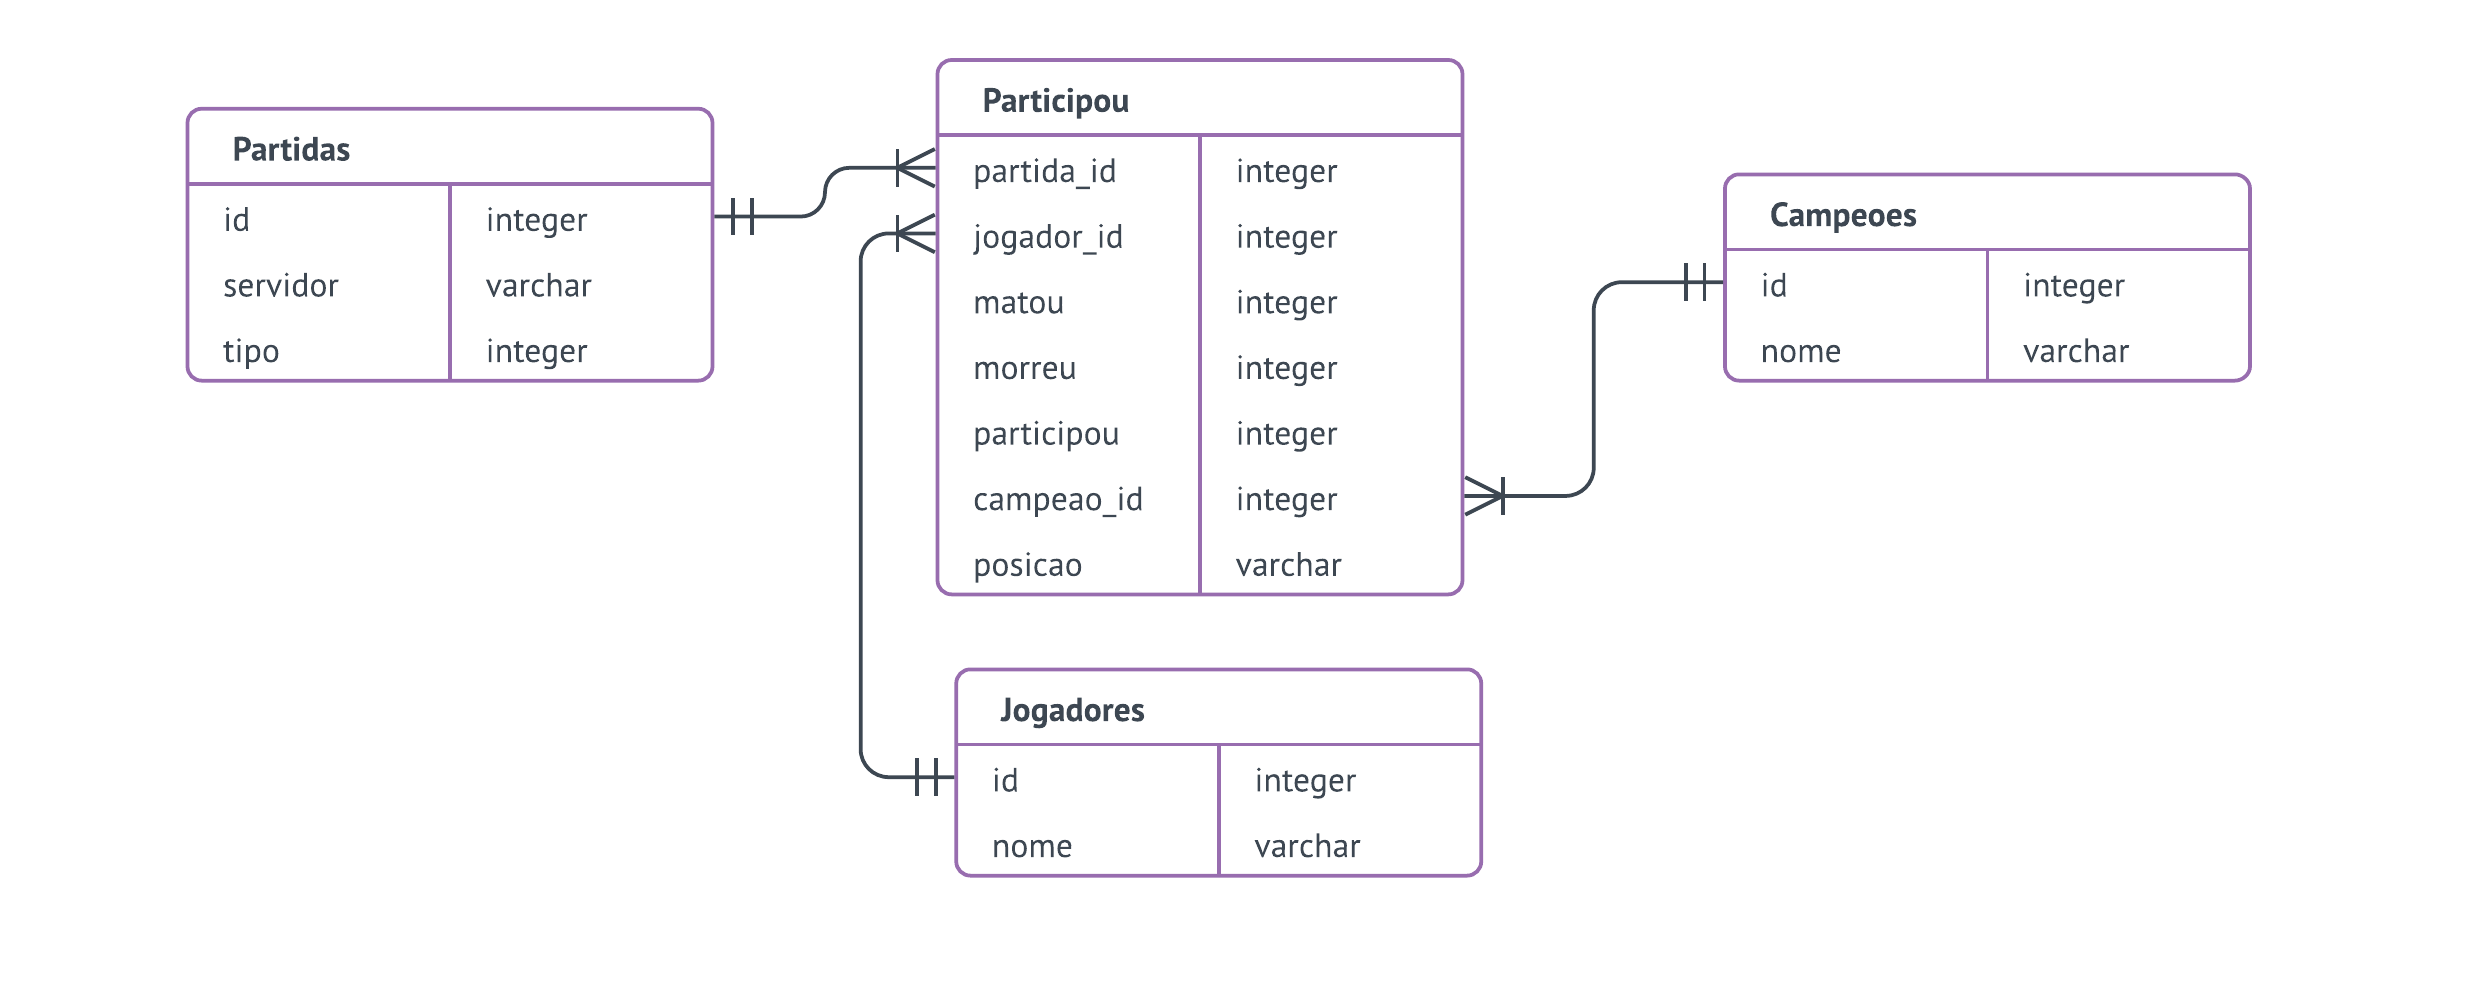
\includegraphics[width=17cm]{imagens/esquema.png}
	\end{center}
	\small{Fonte: Autor.}
	\label{fig:bd}
\end{figure}


\section{Aquisição dos dados}
\label{chap:aquisicao}
A aquisição dos dados será dada à partir de duas fontes: a API da Riot Games; e de um \textit{dataset} público\footnote{https://www.kaggle.com/paololol/league-of-legends-ranked-matches}. Ambos apresentam os mesmos conjuntos de informações em formatos diferentes. Aélm destes, será adquirido outros dados pela API para agilização do trabalho.

A base de dados, na sua versão 9, conta com aproximadamente 183 mil partidas ranqueadas (partidas que, em poucas palavras, servem para classificar as habilidades do jogador) diferentes, dando uma incrementada no banco de dados inicialmente. Estes que precisam ser convertidos para o esquema do banco de dados usados no trabalho.
Em seguida, será usado um algoritmo para a aquisição dos dados de partidas pela API do \textit{League of Legends} em \textit{Python}, que usa a biblioteca \textit{requests} para conseguir acessar a API por URL's, verificando se a partida requisitada existe e se os dados necessários estão completos, salvando no banco de dados apenas as partidas válidas. O pseudo-código se encontra no Algoritmo \ref{alg:main-aqui}.

\
 %Código


\begin{algorithm}[H]
   \SetAlgoLined
     \Inicio{

		i = 1000000000;\tcp*[f]{Esta é a \textit{id} de uma partida aleatória na ultima versão do jogo}
            
		chave = minha chave privada de acesso;
            
        \uSe{Existe arquivo com ultimo partida lido}{
          	i = ultima partida lida;
        }
        \Repita{Até ser pausado}{    
            pedido = requisita URL Da API(i, chave);

            \Se((\tcp*[f]{Se a partida existe}){pedido.status == 200 }{
            	 
            	JSON = carrega JSON Do Pedido(pedido);
                
                \uSe{JSON é válido}{
                	Armazena os dados em um banco de dados;
                }
                
                i = i + 1;

            }
		}
	                
	Salva i no arquivo;
    }
   \label{alg:main-aqui}
   \caption{\textsc{Aquisição dos dados das partidas}}
 \end{algorithm}

\

Decidiu-se usar apenas as partidas ranqueadas 5 contra 5, já que estas são as partidas responsáveis pela classificação dos jogadores dentro dos jogo, e as partidas não ranqueadas são consideradas como amistosas.
Na etapa seguinte são contabilizados quantas vezes cada campeão específico apareceu em uma mesma partida com outro campeão específico, seja no mesmo time ou no time adversário, calculando quantas vitórias em oposição e quantas vitórias em junção.

Com as informações já processadas, foi montado um \textit{web service}, que será explicado na seção \ref{chap:web}, utilizando uma biblioteca chamada D3.js para uma melhor visualização dos dados obtidos , biblioteca essa que será explanado na próxima seção.

\section{Visualização dos dados}
\label{chap:web}

O \textit{web service} será criado utilizando o \textit{framework} Flask, que como \citet[tradução do autor]{flask} diz "Flask é um micro \textit{framework} para Python baseado em Werkzeug, Jinja 2 e em boas intenções.".

Com esse serviço será possível um relatório geral, onde o usuário será capaz de ver a topologia do modelo, vendo quais são os campeões melhores contra os outros e quais são as duplas mais favoráveis, podendo filtrar quais deles podem participar da pesquisa e quais não podem. 
Também será exequível a predição de uma partida, na qual se seleciona os campeões de cada equipe e o sistema tenta antever quem vencerá.



\section{Classificação da topologia}
\label{chap:topo}
Esperando o artigo.

\section{Predição dos dados}
\label{chap:pred}

Para a parte de predição dos dados, serão considerados as conexões e os pesos entre os campeões da partida obtidas através do grafo obtido na Seção \ref{chap:aquisicao}. Os dados de cada partida foram transformados em 3 informações de entrada e a saída:

\begin{itemize}
	\item Sinergia Time 0;
	\item Sinergia Time 1;
	\item Entropia Somada;
	\item Time vencedor.
\end{itemize}

Sendo que as duas primeiras informações se referem a somatória dos pesos da aresta que diz o quão bom os campeões de um time vencem juntos, dados 0 a 1. Para tanto, vamos considerar que\( p_1, p_2, p_3, p_4, p_5 \) são do time 0, \( p_6, p_7, p_8, p_9, p_10 \) do time 1, e \(w(u,v)\) sendo o peso da arestas de porcentagem de partidas ganhas juntas de \(u\) e \(v\), de 0 a 1. Então pode se dizer que: \[ Sinergia Time 0 = \sum_{\overset{1<=i<=5}{i<j<=5}}w(p_i,p_j),\] e, também: \[ Sinergia Time 1 = \sum_{\overset{6<=i<=10}{i<j<=10}}w(p_i,p_j).\]

A entropia somada, foi definida como a soma de quantas partidas um campeão \(c_1\) ganhou de um campeão \(c_2\), sendo que este valor também vai de 0 a 1. A definição matemática pode ser descrita como, sendo \(w_e(c_1,c_2)\) a porcentagem que o \(c_1\) ganhou do \(c_2\) : \[ Entropia Somada = \sum_{\overset{1<=i<=5}{6<=j<=10}}w_e(c_i,c_j)\]

A entropia do time 1 para o time 0 não foi feita, porque a correlação entre as duas entropias seria alta, uma vez que \(w_e(p_i, p_j) = 1 - w_e(p_j, p_i)\) e elas informariam a mesma coisa. Então, por eficiência, e para aumentar a velocidade de treino do modelo, ela foi retirada. O time vencedor apenas diz qual time venceu, informando se foi o time 0 ou o time 1.

Então com esses valores, é criado um classificador KNN, em que, com as três informações de entrada, ele tentará classificar o time vencedor. Os valores que foram armazenados, são separados em dados de treino e de teste, sendo que o teste representam 20\% dos dados totais e todos os dados são re-escalados no intervalo de 0 a 1, para que o KNN possa ser treinado adequadamente.
Com o modelo final treinado e testado, o \textit{webservice} será capaz de comunicar com o KNN para responder às entradas do usuário, indicando um time vencedor.
\
\chapter{Resultados}

O trabalho ficou quatro meses adquirindo partidas da API do LOL, sendo que apenas 14 mil partidas aproximadamente eram válidas para os filtros descritos na Seção \ref{chap:aquisicao} que dizem que as partidas devem ser ranqueadas e não terem os dados incompletos.
Por este algoritmo, foram armazenadas \numpartidas\ jogos válidos diferentes, com esse escopo e o número de partidas usados foram ao todo \partidasrankeds\, contando com o \textit{dataset} público.
Na tabela \ref{tab:subset-lol} é possível ver uma pequena fatia dos dados salvos.


\begin{table}[H]
	\centering
	\caption{Exemplo de \textit{subset} salvo no banco de dados}
	\label{tab:subset-lol}
	\resizebox{\textwidth}{!}{%
		\begin{tabular}{cccccccccc}
			match\_id  & kills & deaths & assists & win & champ\_id & lane   & player\_id & platform & type \\
			1282000002 & 11    & 10     & 7       & 0   & 67        & BOTTOM & 16112724   & BR1      & 420  \\
			1282000002 & 2     & 8      & 15      & 0   & 412       & BOTTOM & 18604874   & BR1      & 420  \\
			1282000002 & 7     & 4      & 7       & 0   & 34        & MIDDLE & 19281809   & BR1      & 420  \\
			1282000002 & 7     & 6      & 4       & 0   & 5         & JUNGLE & 21304223   & BR1      & 420  \\
			1282000002 & 5     & 7      & 12      & 0   & 98        & TOP    & 651014     & BR1      & 420  \\
			1282000002 & 0     & 6      & 23      & 1   & 44        & BOTTOM & 18592234   & BR1      & 420  \\
			1282000002 & 19    & 5      & 5       & 1   & 222       & BOTTOM & 7170345    & BR1      & 420 
		\end{tabular}%
	}
	\small{Fonte: Autor.}
\end{table}

Com os dados armazenados, e o processamento deles executado, foi feito o \textit{webservice} que consegue exibir para o usuário as informações sobre a topologia do grafo, qual campeão é adequado contra um outro específico.
Na Figura \ref{fig:web_service_relatorio} é possível ver um exemplo de uso do serviço para uma visão geral das informações e na Figura \ref{fig:topologiawebservice} mostra quem tem uma sinergia com quem (arestas verdes) e quem é um \textit{counter pick} do outro (arestas com uma seta vermelha orientando o grafo). O tamanho das arestas dos campeões indica a quantidade de vezes que que aquele determinado herói jogou com os filtros escolhidos pelo usuário.



\begin{figure}[H]
	
	\centering
	\caption{Exemplo de uso do \textit{web service} para visão geral dos dados.}
	\subfloat[Filtro dos dados para campeões da mesma equipe.]{
		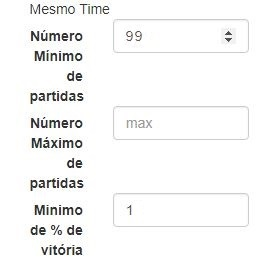
\includegraphics[width=0.4\textwidth]{imagens/web_1.JPG}
	}
	\subfloat[Filtro dos dados para adversários.]{
		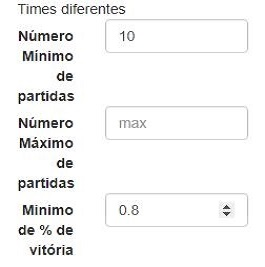
\includegraphics[width=0.4\textwidth]{imagens/web_2.JPG}
	}
	\qquad
	\subfloat[Filtro para escolher quais campeões podem participar (\textit{picks}) e quais nao podem (\textit{bans}).]{
		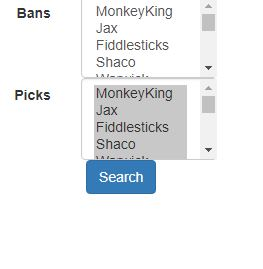
\includegraphics[width=0.4\textwidth]{imagens/web_3.JPG}
	}
	\subfloat[Exemplo de grafo exibido pelo \textit{web service}, sendo as setas vermelhas mostrando quem é bom contra quem, e as linhas continuas quem é bom com quem. O tamanho do circulo é a frequência daquela ligação e a cor é a força da ligação.]{
		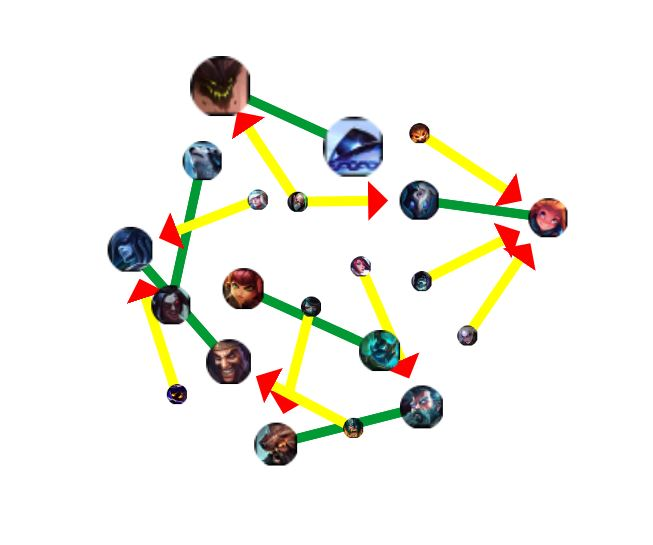
\includegraphics[width=0.4\textwidth]{imagens/web_4.JPG}
		\label{fig:topologiawebservice}
	}
	
	\small{Fonte: Autor.}
	\label{fig:web_service_relatorio}
\end{figure}


É possível ver topologia da rede complexa final na Figura \ref{fig:cnfinal}, que consta com 139 vértices diferentes ( todos os heróis lançados até a aquisição dos dados ) e com 19180 arestas já que estas são orientadas, e que se aproxima de uma rede mundo pequeno, pois faltam duas arestas para se tornar uma rede regular.

\begin{figure}[H]
	\caption{Visualização da topologia final da Rede Complexa.}
	\begin{center}
		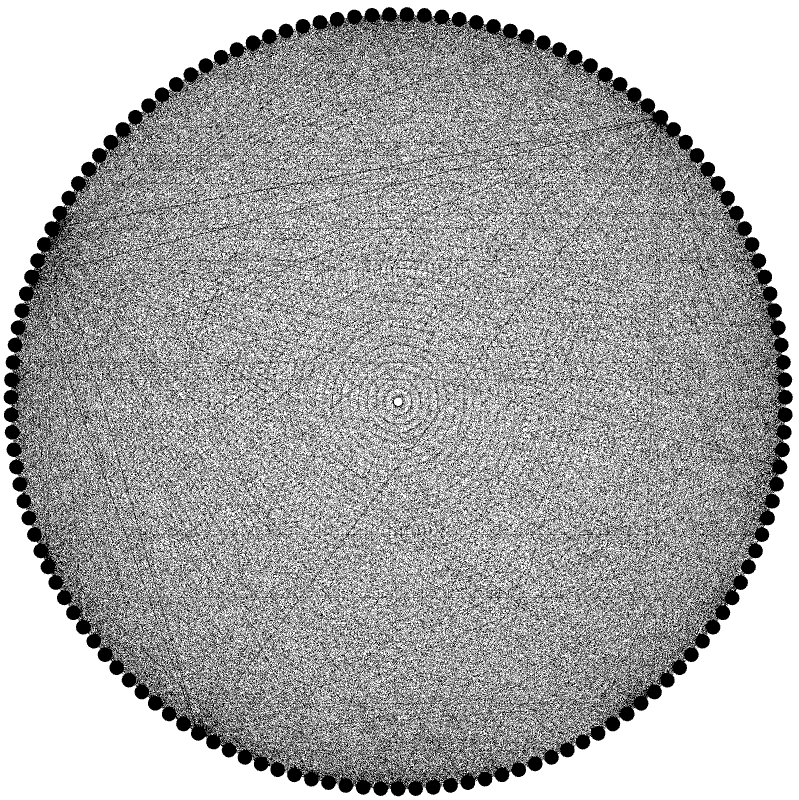
\includegraphics[width=1\textwidth]{imagens/grafofinal.png}
	\end{center}
	\small{Fonte: Autor.}
	\label{fig:cnfinal}
\end{figure}

\begin{figure}[H]
	\caption{Erro do KNN em variação ao K.}
	\begin{center}
		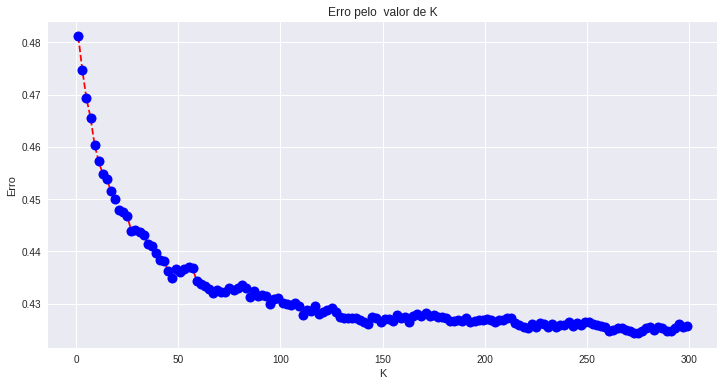
\includegraphics[width=1\textwidth]{imagens/knn.png}
	\end{center}
	\small{Fonte: Autor.}
	\label{fig:KNNgrafico}
\end{figure}


O Classificador KNN ficou com uma precisão de 58\% com a melhor calibração conseguida, com o \(k = 243\), na Figura \ref{fig:KNNgrafico} é possível ver a precisão em relação ao \(k\). E com o modelo preparado é possível entrar no \textit{webservice} e selecionar os campeões de cada time e conferir o resultado da predição. É possível ver um exemplo de uso do \textit{webservice} na Figura \ref{fig:predicaowebservice} onde possível ver a sinergia dos dois times e a entropia da partida.

Com a matriz de confusão é possível ver as classificações corretas e as erradas por resultado, ou seja, na Tabela \ref{tab:confusion} é possível ver quantas vezes o KNN classificou sendo vencedor o time 0, porém era vencedor o time 1 ou qualquer outro cenário.

\begin{table}[]
	\centering
	\caption{Matriz de confusão do KNN}
	\label{tab:confusion}
		\resizebox{\textwidth}{!}{%
\begin{tabular}{|c|c|c|}
	\hline
	Real x Predição & time 0 & time 1 \\ \hline
	time 0          & 10909  & 6993   \\ \hline
	time 1          & 7848   & 9107   \\ \hline
\end{tabular}
}
\
\
\small{Fonte: Autor.}
\end{table}


\begin{figure}[H]
	
	\centering
	\caption{Exemplo de uso do \textit{webservice} predição da partida}
	\subfloat[Área para escolher o time 0.]{
		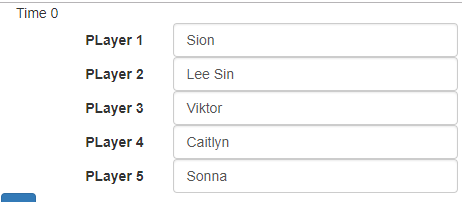
\includegraphics[width=0.4\textwidth]{imagens/predict_1.PNG}
	}
	\subfloat[Área para escolher o time 1.]{
		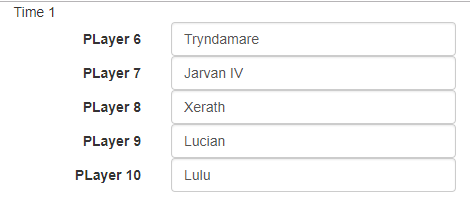
\includegraphics[width=0.4\textwidth]{imagens/predict_2.PNG}
	}
	\qquad
	\subfloat[Exemplo de resposta do \textit{webservice}.]{
		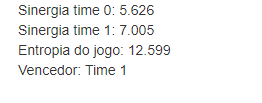
\includegraphics[width=0.4\textwidth]{imagens/predict_3.PNG}
	}
	\subfloat[Tela toda da parte de predição.]{
		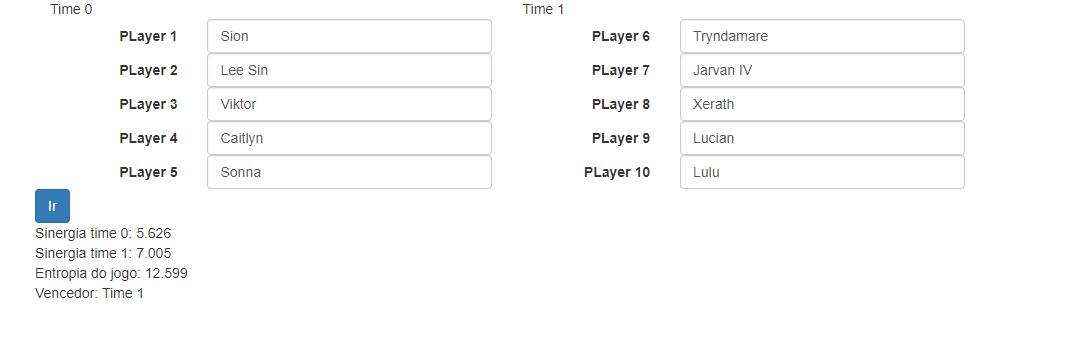
\includegraphics[width=0.4\textwidth]{imagens/predict_4.PNG}
	}
	
	
	\small{Fonte: Autor.}
	\label{fig:predicaowebservice}
\end{figure}
\
\chapter{Conclusão}

\begin{figure}[H]
	
	\centering
	\caption{Exemplo de uso do \textit{web service} predição da partida}
	\subfloat[Esperando ser feito]{
		\rule{7cm}{7cm}
	}
	\subfloat[Esperando ser feito]{
		\rule{7cm}{7cm}
	}
	\qquad
	\subfloat[Esperando ser feito]{
		\rule{7cm}{7cm}
	}
	\subfloat[Esperando ser feito]{
		\rule{7cm}{7cm}
	}
	
	
	\small{Fonte: Autor.}
	\label{fig:web_service_predict}
\end{figure}

\setlength{\baselineskip}{\baselineskip}

%%=============================================================================
%% Referências
%%=============================================================================
\begin{flushleft}
\bibliographystyle{abnt}
\bibliography{referencias/referencias}
\end{flushleft}

%IMPORTANTE: Se precisar usar alguma seção ou subseção dentro dos apêndices ou
%anexos, utilizar o comando \tocless para não adicionar no Sumário
%Exemplos: 
% \tocless\section{Histórico}
%%=============================================================================
%% Apêndices
%%=============================================================================
%\appendix

%%IMPORTANTE: Se precisar usar alguma seção ou subseção dentro dos apêndices ou
%anexos, utilizar o comando \tocless para não adicionar no Sumário
%Exemplos: 
% \tocless\section{Histórico}
% \tocless\subsection{Detalhes}
\tocless\section{teste}
%Este é um teste de seção dentro do apêndice


%\chapter{Título do apêndice Ex}
Esta é o apêndice B



%%=============================================================================
%% Anexos
%%=============================================================================
%\annex
%\chapter{Título do Anexo}
Este é o anexo A



\end{document}
